\section{Funktionenfolgen}
\begin{definition}
  Eine Funtionenfolge ist allgemein eine Folge von Funktionen $f_1, f_2, ...$ bei denen alle Funktion dieselbe Definitions- und Zielmenge haben.
  \begin{equation}
  f:D\times \N \rightarrow Z, \quad (x,n) \rightarrow f_n(x)
  \end{equation}
  Wobei $D$ die Definitionsmenge und $Z$ die Zielmenge ist.
\end{definition}
\begin{definition}
  \begin{itemize}
    \item[a )] Eine Folge von Funktionen $f_n$ mit $f_n: D \rightarrow \R$ mit $D \subset \R$ heißt für $n \rightarrow \infty$ punktweise gegen $f$ konvergent, falls für alle $x \in D: \lim\limits_{n \rightarrow \infty} f_n(x) = f(x)$ gilt.
    \item[b )] Eine Funktionenfolge heißt gleichmäßig konvergent, falls \newline $\lim\limits_{n \rightarrow \infty} \sup\limits_{x \in D} |f_n(x) -f(x)| = 0$ gilt.
  \end{itemize}
  \begin{figure}[H] 
		\centering
	  \centering
	  \captionsetup{justification=centering}
	  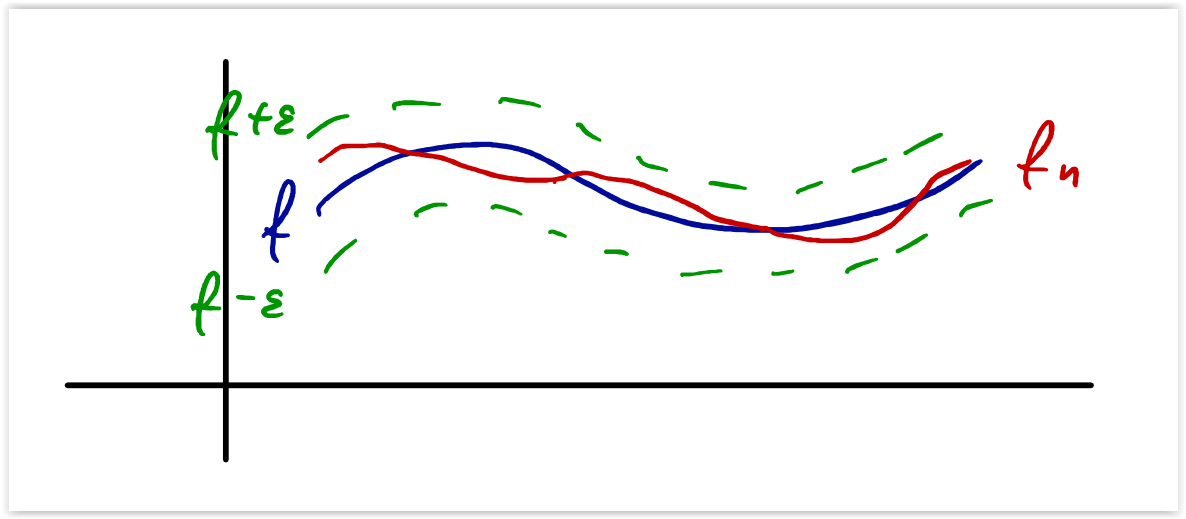
\includegraphics[width=0.5\linewidth]{./img/funktionenfolgen_konvergenz.png}
	  \caption{Epsilonkanal Funktionenfolge \protect\cite{HM12}}
	  \label{fig:funktionenfolge_konvergenz}
  \end{figure}
\end{definition}
\begin{satz}
  Gegeben sei eine Folge stetiger Funktionen mit $f_n: D\rightarrow \R$. Gilt $f_n \rightarrow f$ gleichmäßig auf $D$, so ist auch die Grenzfunktion stetig.
\end{satz}
\begin{satz}
  Zu jeder Potenzreihe gibt es den Konvergenzradius $r$ mit $0 \leq r \leq \infty$ mit der Eigenschaft, dass $\sum\limits_{k=0}^\infty a_k(z-z_0)^k$ absolut konvergent für $|z-z_0| < r$ und divergent für $|z-z_0|>r$ ist.\newline
  Ferner konvergiert die Potenzreihe auf jeder Kreisscheibe $|z-z_0| < \delta$ mit $\delta < r$ auch gleichmäßig. 
\end{satz}
\begin{bem}
  Die Konsequenz aus obigem Satz ist, dass Potenzreihen für alle $z$ mit $|z-z_0| < r$ stetig sind.
\end{bem}
\begin{satz}
  $(f_n)_{n \in \N}$ seien auf $[a,b]$ differenzierbar. Für ein $x_0 \in [a,b]$ sei $f_n(x_0)$ konvergent. Ferner konvergiere $(f'_n)_{n \in \N}$ gleichmäßig (gegen $g$) auf $[a,b]$. Dann gilt:
  \begin{itemize}
    \item[1) ] $(f_n)_{n \in \N}$ konvergiert auf $[a,b]$ gleichmäßig.
    \item[2) ] $f(x) = \lim\limits_{n \rightarrow \infty} f_n(x)$ ist differenzierbar auf $[a,b]$ und es gilt $f'(x) = \lim\limits_{n \rightarrow \infty} f_n'(x)$ (und es gilt $f' = g$).
  \end{itemize}
\end{satz}
\begin{bem}
  Die Konsequenz aus obigem Satz ist, dass Potenzreihen innerhalb ihres Konvergenzradius beliebig oft differenzierbar sind und gliedweise abgeleitet werden können.
\end{bem}
\newpage